\documentclass[tikz,border=2]{standalone}
\usetikzlibrary{shadows,arrows,shapes,positioning,calc,backgrounds,fit}
\newcommand{\vanish}[1]{}
\usepackage{array}
\newcommand{\calc}[1]{\mbox{$\mathcal{C}_{#1}$}}
\usepackage{ctable}
\pdfpageattr {/Group << /S /Transparency /I true /CS /DeviceRGB>>}
% Define the layers to draw the diagram
%
\begin{document}
%% \pgfdeclarelayer{bg}
%% \pgfdeclarelayer{fg}
%% \pgfsetlayers{bg,main,fg}
%
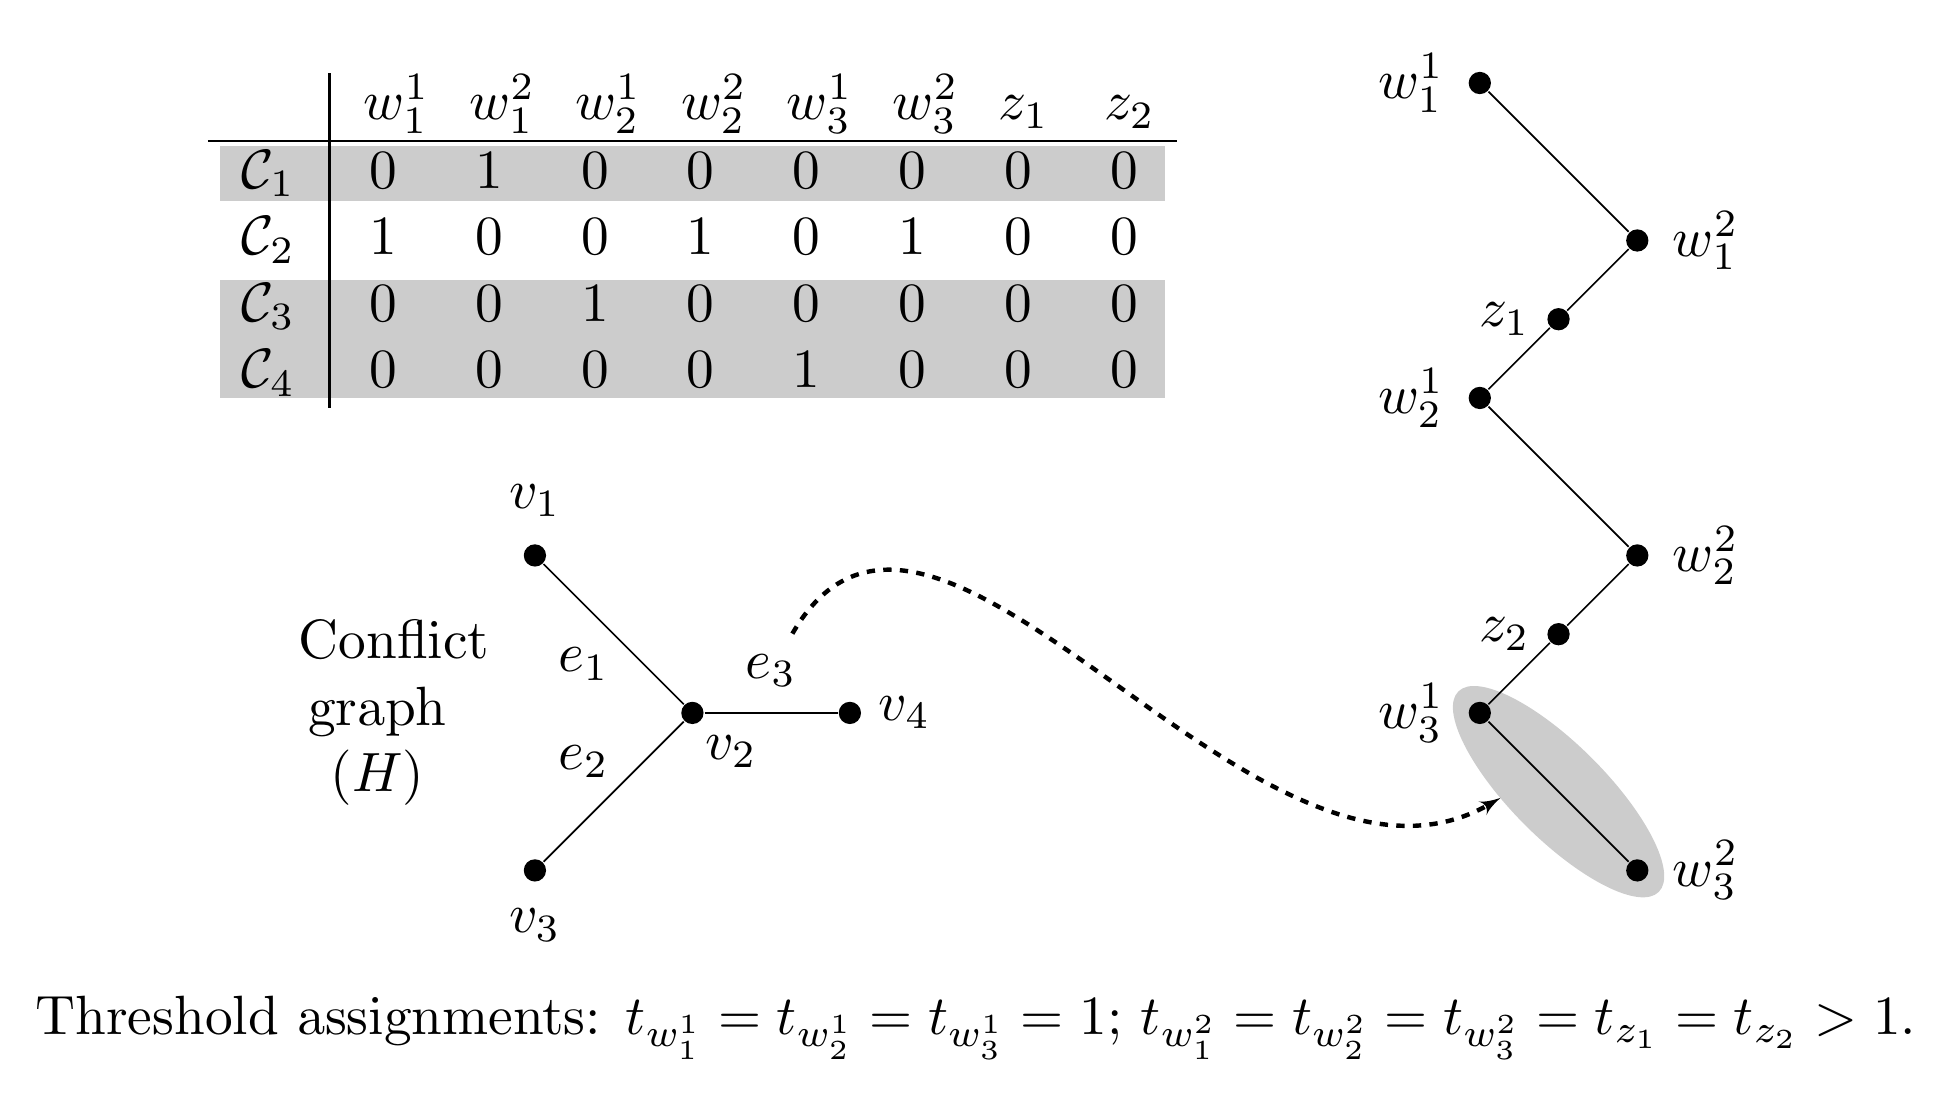
\begin{tikzpicture}
[scale=2,node distance=.5cm, transform shape,
every node/.style={shape=circle,fill,inner sep=.5mm},
myblock/.style={draw=none,fill=none,scale=1.5,inner sep=0pt},
myedge/.style={>=latex', shorten >=.0pt, shorten <=.0pt,semithick},
every fit/.style={fill=black!10,ellipse,draw=black!20},
myellipse/.style={fill=black!20,draw=none}]
%%%%%%%%%%
%%%%% The configurations
\begin{scope}[shift={(0,0)}]
\node [draw=none, fill=none, shape=rectangle,scale=1] at (0,0) {
   \begin{tabular}{c|>{\centering\arraybackslash}p{2.5mm}>{\centering\arraybackslash}p{2.5mm}>{\centering\arraybackslash}p{2.5mm}>{\centering\arraybackslash}p{2.5mm}>{\centering\arraybackslash}p{2.5mm}>{\centering\arraybackslash}p{2.5mm}>{\centering\arraybackslash}p{2.5mm}>{\centering\arraybackslash}p{2.5mm}}
        & $w_1^1$ & $w_1^2$ & $w_2^1$ & $w_2^2$ & $w_3^1$ & $w_3^2$ & $z_1$ & $z_2$\\\hline
        $\mathcal{C}_{1}$ & $0$ & $1$ & $0$ & $0$ & $0$ & $0$ & $0$ & $0$ \\
        $\mathcal{C}_{2}$ & $1$ & $0$ & $0$ & $1$ & $0$ & $1$ & $0$ & $0$ \\
        $\mathcal{C}_{3}$ & $0$ & $0$ & $1$ & $0$ & $0$ & $0$ & $0$ & $0$ \\
        $\mathcal{C}_{4}$ & $0$ & $0$ & $0$ & $0$ & $1$ & $0$ & $0$ & $0$
    \end{tabular}
};
   \begin{pgfonlayer}{background}
      \draw[myellipse,shift={(-3,.25)}] (0,0) rectangle (6,.35);
      \draw[myellipse,shift={(-3,-1)}] (0,0) rectangle (6,.75);
   \end{pgfonlayer}
\end{scope}
%%
%%%%% The underlying graph
\begin{scope}[shift={(5,1)}]
   \node (w11) [label=left:$w_1^1$] at (0,0) {};
   \node (w12) [label=right:$w_1^2$] at (1,-1) {};
   \node (z1) [label=left:$z_1$] at (.5,-1.5) {};
   \node (w21) [label=left:$w_2^1$] at (0,-2) {};
   \node (w22) [label=right:$w_2^2$] at (1,-3) {};
   \node (z2) [label=left:$z_2$] at (.5,-3.5) {};
   \node (w31) [label=left:$w_3^1$] at (0,-4) {};
   \node (e3d) [fill=none] at (.2,-4.5) {};
   \node (w32) [label=right:$w_3^2$] at (1,-5) {};
   \path[draw,myedge] (w11) -- (w12) -- (z1) -- (w21) -- (w22) -- (z2) --
   (w31) -- (w32);
   \begin{pgfonlayer}{background}
      \draw[myellipse] ellipse[xshift=.5cm,yshift=-4.5cm,x radius=.9cm,y
      radius=.3cm, rotate=-45];
   \end{pgfonlayer}
\end{scope}
%%
%%%%% The conflict graph
\begin{scope}[shift={(-1,-2)}]
   \node (v1) [label=above:$v_1$] at (0,0) {};
   \node (v2) [label=below right:$v_2$] at (1,-1) {};
   \node (v3) [label=below:$v_3$] at (0,-2) {};
   \node (v4) [label=right:$v_4$] at (2,-1) {};
   \draw[myedge] (v1) -- (v2) node [fill=none,below left,midway] {$e_1$};
   \draw[myedge] (v2) -- (v4) node (e3) [fill=none,above,midway] {$e_3$};
   \draw[myedge] (v2) -- (v3) node [fill=none,above left,midway] {$e_2$};
   \node [fill=none] at (-1,-1) {\parbox{1cm}{\centering Conflict graph
   ($H$)}};
\end{scope}
\draw[dashed,myedge,->,ultra thick] (e3)
edge[out=60,in=-150,looseness=1] (e3d);
\node at (1.8,-5) [rectangle,fill=none,minimum height=0pt] {Threshold assignments:
   $t_{w_1^1}=t_{w_2^1}=t_{w_3^1}=1$;
   $t_{w_1^2}=t_{w_2^2}=t_{w_3^2}=t_{z_1}=t_{z_2}>1$.};
\end{tikzpicture}
\end{document}
